\documentclass[11pt,a4paper]{article}

\usepackage[T1]{fontenc}
\usepackage[utf8]{inputenc}
\usepackage[spanish,es-noshorthands,es-tabla]{babel}
\usepackage{newpxtext,newpxmath}
\usepackage[a4paper,top=2.5cm,bottom=2.5cm,left=2.6cm,right=2.6cm,headheight=14pt]{geometry}
\usepackage{microtype}
\usepackage{graphicx}
\usepackage{booktabs}
\usepackage{siunitx}
\usepackage{amsmath}
\usepackage{xcolor}
\usepackage[font=small,labelfont=bf,labelsep=period]{caption}
\usepackage{enumitem}
\usepackage{fancyhdr}
\usepackage{titlesec}
\usepackage[hidelinks]{hyperref}

\graphicspath{{figuras/}}
\sisetup{output-decimal-marker={,}, group-digits=false, per-mode=symbol, detect-all}
\setlist{itemsep=3pt, topsep=4pt, leftmargin=*}
\setlength{\parskip}{4pt}
\setlength{\parindent}{0pt}
\definecolor{acento}{HTML}{1F4E79}

\titleformat{\section}{\large\bfseries\color{acento}}{\thesection.}{0.6em}{}
\titleformat{\subsection}{\normalsize\bfseries}{\thesubsection.}{0.6em}{}
\titlespacing*{\section}{0pt}{14pt}{6pt}
\titlespacing*{\subsection}{0pt}{10pt}{4pt}

\pagestyle{fancy}
\fancyhf{}
\fancyhead[L]{\small\color{gray}P2. Sistemas propulsivos}
\fancyhead[R]{\small\color{gray}Eden Rochman Sharabi}
\fancyfoot[C]{\small\thepage}
\renewcommand{\headrulewidth}{0.4pt}

\newcommand{\Uoc}{U_{\mathrm{OC}}}

\begin{document}
\thispagestyle{plain}
\begin{center}
  {\small\color{gray}Sistemas y Subsistemas de Aeronaves no Tripuladas (UAS)\\
  Universitat Politècnica de València}\\[10pt]
  {\LARGE\bfseries Práctica 2: Ensayo de sistemas propulsivos}\\[6pt]
  {\large Motor eléctrico en vacío (sin hélice)}\\[10pt]
  {\large Eden Rochman Sharabi}
\end{center}
\vspace{4pt}
{\color{acento}\hrule height 0.8pt}
\vspace{6pt}

\section{Objetivo y montaje}
Se caracteriza un motor eléctrico sin hélice. Una Raspberry Pi Pico 2 genera la señal PWM (\SI{50}{\hertz}, pulso de 1 a \SI{2}{\milli\second}) que gobierna el ESC, alimentado por una batería 6S. El ESC conmuta las tres fases del motor. Se miden las rpm con un sensor Jeti y con el osciloscopio PicoScope, y la corriente con una resistencia shunt (\SI{20}{\ampere}/\SI{100}{\milli\volt}, es decir, \SI{5}{\milli\ohm}). Las medidas las tomó el grupo de prácticas; el procesado está en \texttt{P2\_analisis.py}.

\section{Parte 1: subsistemas}
\begin{table}[h]
  \centering
  \caption{Características de los subsistemas.}
  \begin{tabular}{l l r}
    \toprule
    Subsistema & Magnitud & Valor \\
    \midrule
    Batería 6S & Tensión & \SI{24.8}{\volt} \\
               & Capacidad & \SI{3.3}{\ampere\hour} \\
               & Energía ($24{,}8\times 3{,}3$) & \SI{81.8}{\watt\hour} \\
               & $I_{max}$ & \SI{10}{\ampere} \\
               & $P_{max}$ ($24{,}8\times 10$) & \SI{248}{\watt} \\
    \midrule
    ESC        & Rango de tensión & \SIrange{18}{50.4}{\volt} \\
               & Intensidad continua / máxima & \SI{60}{\ampere} / \SI{80}{\ampere} \\
               & $P_{max}$ ($80\times 50{,}4$) & \SI{4032}{\watt} \\
    \midrule
    Motor F2004 & Tipo & brushless outrunner \\
               & Configuración & 12N14P (12 ranuras, 14 polos) \\
               & Constante $K_v$ & \SI{1700}{rpm/\volt} \\
               & Tensión recomendada & 6S \\
               & Intensidad máxima & \SI{21.2}{\ampere} \\
               & $P_{max}$ (\SI{60}{\second}) & \SI{503}{\watt} \\
               & Resistencia interna & \SI{221}{\milli\ohm} \\
               & Corriente en vacío (10 V) & \SI{0.38}{\ampere} \\
               & Masa (con cable) & \SI{16.4}{\gram} \\
    \bottomrule
  \end{tabular}
\end{table}
El motor es un T-Motor F2004 KV1700; el modelo se lee en la campana del motor. La configuración y la masa coinciden en las tiendas consultadas; la intensidad y potencia máximas, la resistencia y la corriente en vacío proceden de fichas de distribuidores, no de una hoja oficial de T-Motor, que no he podido consultar. La rotulación del ESC no es legible en las fotos, así que sus datos son los del grupo.

\clearpage
\section{Parte 2: señales en el osciloscopio}
Las figuras muestran la salida PWM de la Pico a 20, 40 y \SI{60}{\percent}: pulsos de \SI{3.3}{\volt} con periodo de \SI{20}{\milli\second}, es decir \SI{50}{\hertz}. El ancho del pulso crece con el porcentaje, que mueve el pulso dentro del intervalo de 1 a \SI{2}{\milli\second}.
\begin{figure}[h]
  \centering
  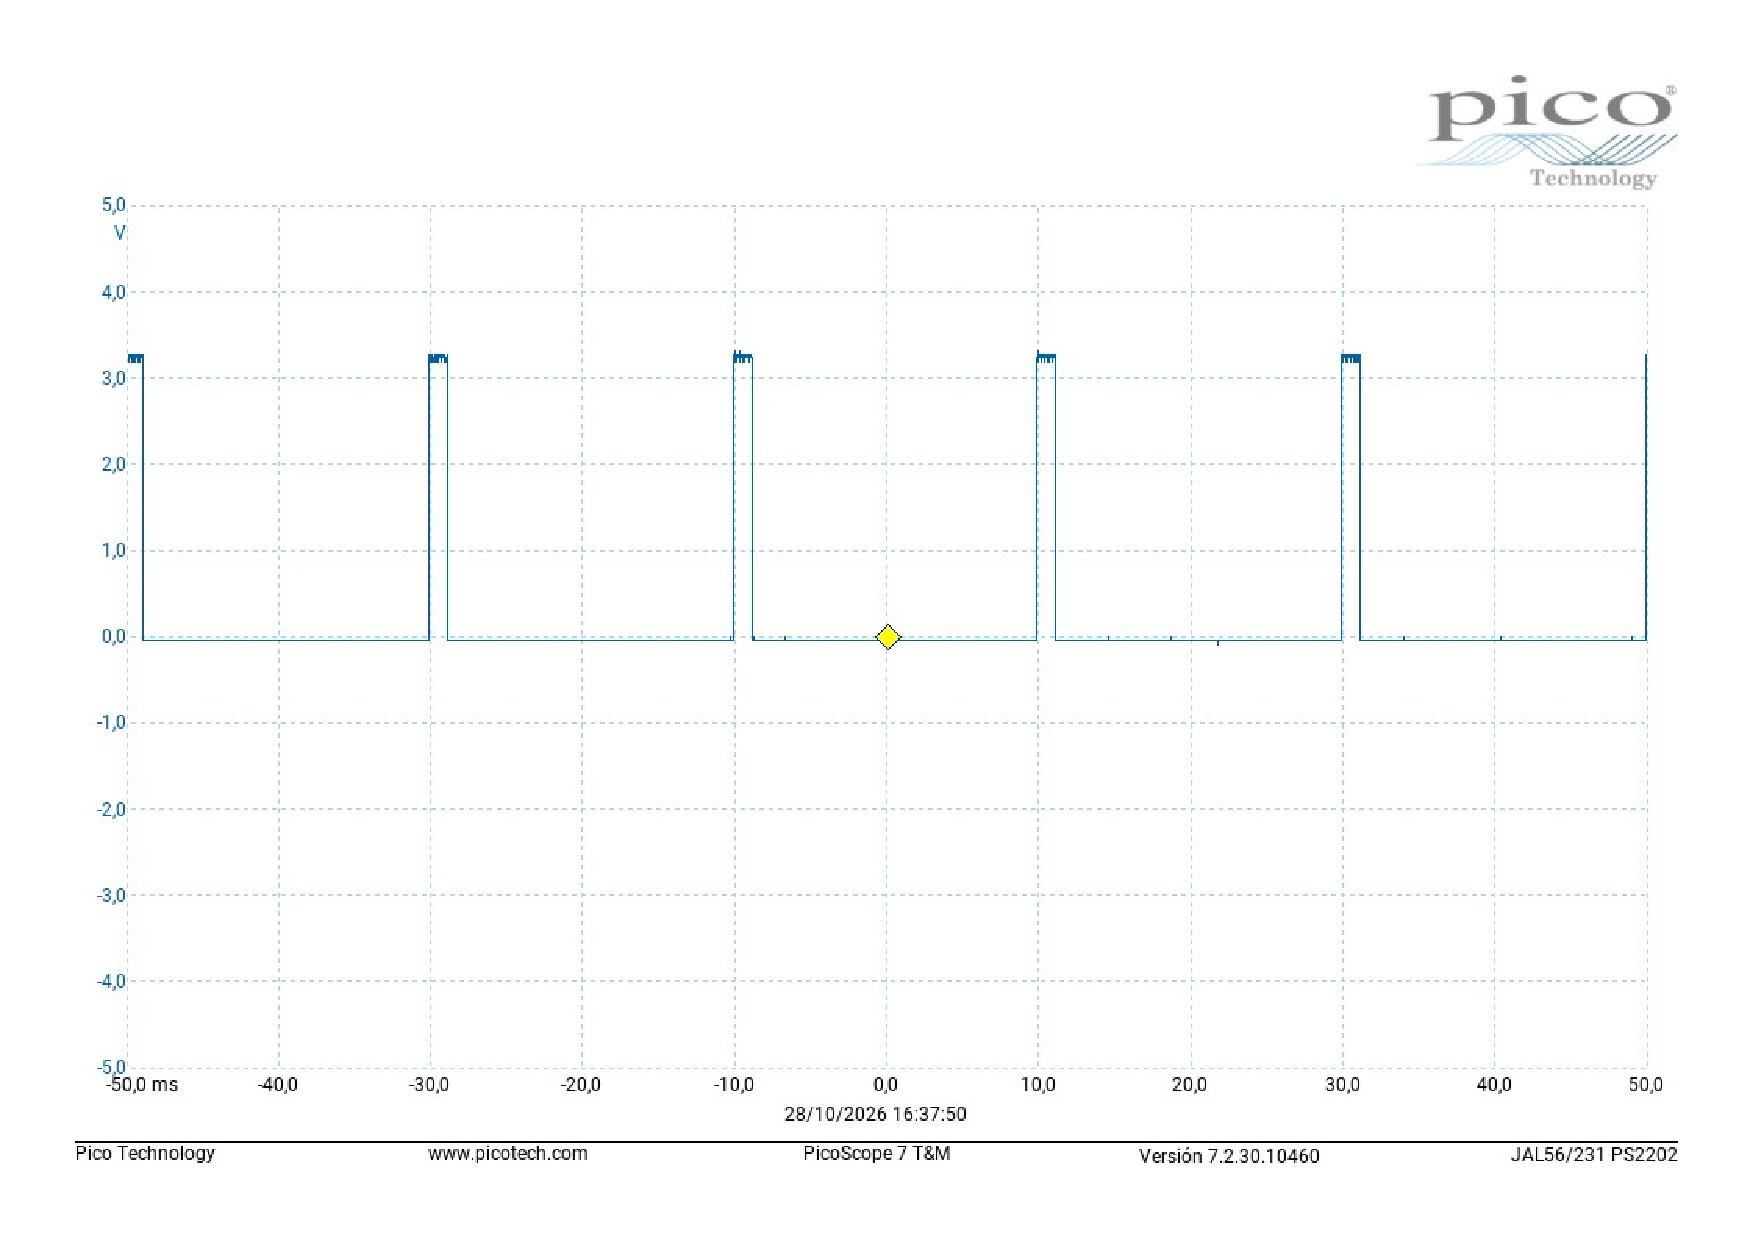
\includegraphics[page=1,width=0.49\textwidth]{pwm_20}\hfill
  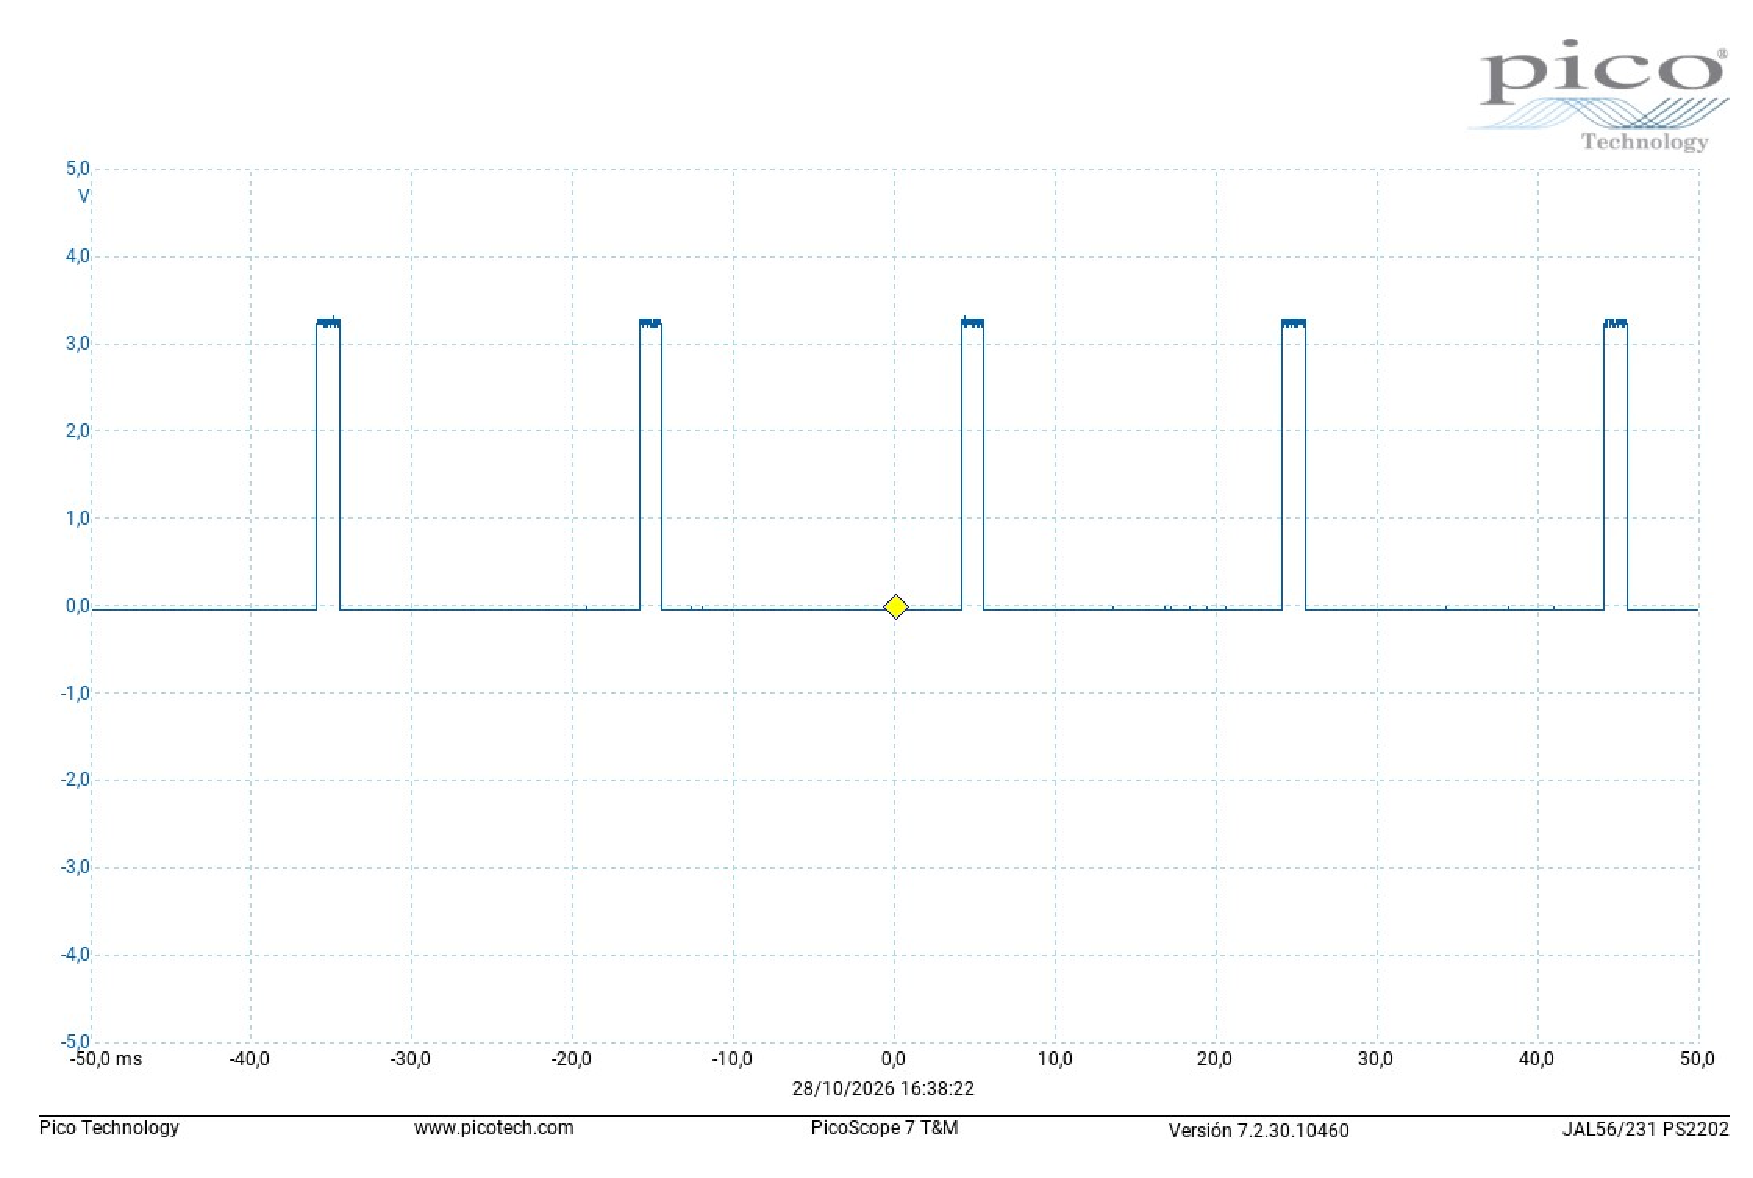
\includegraphics[page=1,width=0.49\textwidth]{pwm_40}\\[4pt]
  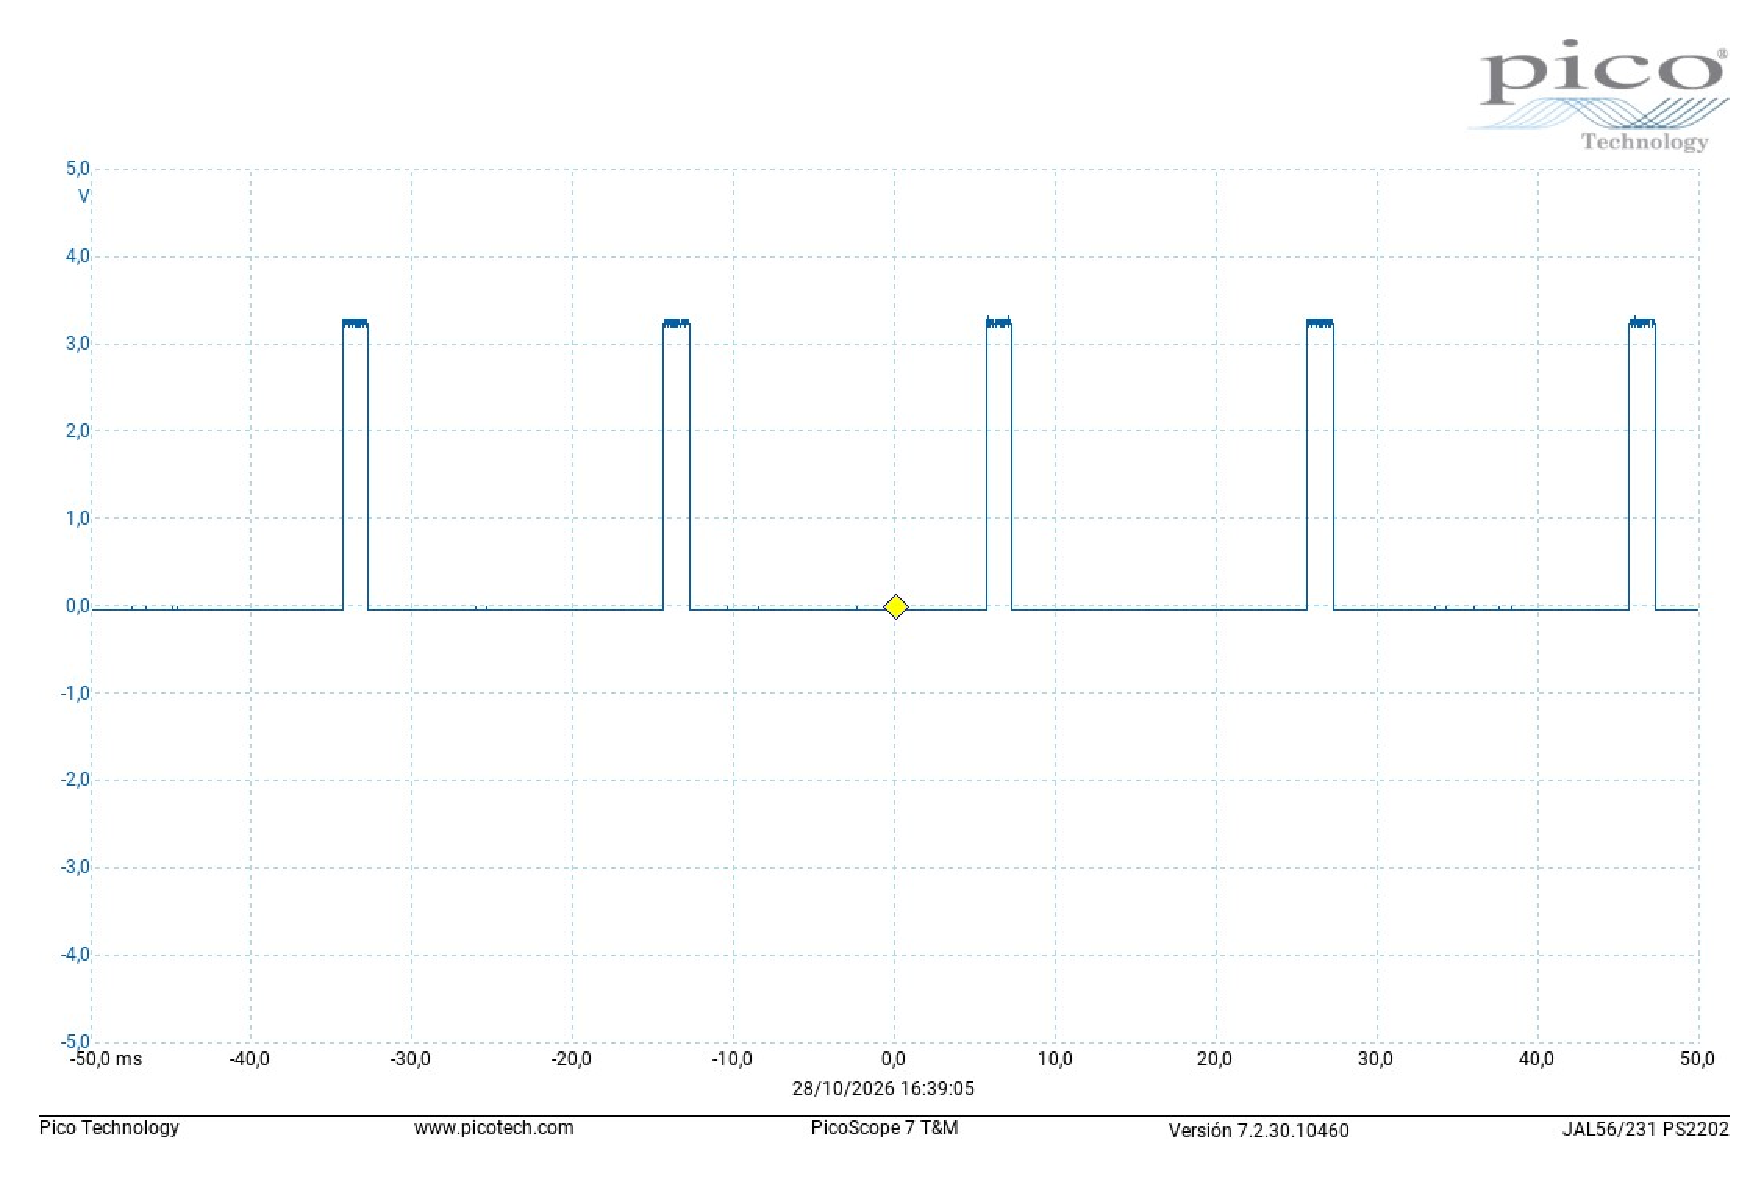
\includegraphics[page=1,width=0.49\textwidth]{pwm_60}
  \caption{Señal PWM de control a 20, 40 y \SI{60}{\percent}.}
\end{figure}
La tensión entre fases y su transformada de Fourier se resumen en $f_{osc}$ (tabla de la Parte 3) y $f_{Fourier}$ (no está en la tabla; la FFT está en el Excel del grupo) ambas coinciden en menos de un \SI{11}{\percent}, y al \SI{20}{\percent} en un \SI{1}{\percent}. Las capturas de las fases no se han facilitado, así que no se incluyen sus figuras.

\section{Parte 3: motor en vacío}
La frecuencia de la señal conmutada es la eléctrica. Con $p$ pares de polos, $\mathrm{rpm} = 60 f / p$. La corriente sale de la caída media en la shunt y la potencia de $P = I\,V_{bat}$ con $V_{bat}=\SI{24.8}{\volt}$:
\begin{equation}
  I = \frac{V_{sh}}{R_{sh}}, \qquad P = I\,V_{bat}.
\end{equation}
El cociente $60f/\mathrm{rpm}_{Jeti}$ vale \num{7.09}, \num{6.91} y \num{6.91} a 20, 30 y \SI{40}{\percent}, así que $p=7$ (\textbf{14 polos}), que coincide con la configuración 12N14P del fabricante. Con $p=7$ se estiman las rpm en todo el rango.

\begin{table}[h]
  \centering
  \caption{Motor en vacío.}
  \begin{tabular}{r S[table-format=4.0] S[table-format=1.2] S[table-format=5.0] S[table-format=5.0] S[table-format=2.1] S[table-format=-1.1]}
    \toprule
    {PWM (\%)} & {$f_{osc}$ (Hz)} & {$I$ (A)} & {rpm osc.} & {rpm Jeti} & {$P$ (W)} & {Error (\%)} \\
    \midrule
    20 & 1280 & 0.25 & 10971 & 10830 & 6.2  & 1.3 \\
    30 & 1728 & 0.36 & 14811 & 15000 & 8.9  & -1.3 \\
    40 & 2247 & 0.43 & 19260 & 19500 & 10.7 & -1.2 \\
    50 & 2598 & 0.52 & 22269 & {--}  & 12.9 & {--} \\
    60 & 3199 & 0.54 & 27420 & {--}  & 13.4 & {--} \\
    70 & 3634 & 0.56 & 31149 & {--}  & 13.9 & {--} \\
    80 & 4485 & 0.58 & 38443 & {--}  & 14.4 & {--} \\
    \bottomrule
  \end{tabular}
\end{table}
\begin{figure}[h]
  \centering
  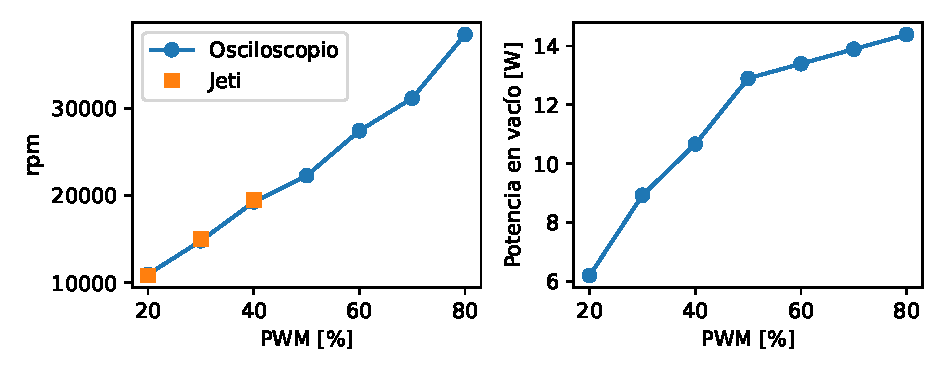
\includegraphics[width=\textwidth]{fig_motor}
  \caption{rpm y potencia en vacío frente al PWM.}
\end{figure}
\begin{itemize}
  \item El osciloscopio reproduce al Jeti con un error de $\pm\SI{1.3}{\percent}$ (20--\SI{40}{\percent}), lo que valida $p=7$. A \SI{24.8}{\volt} y $K_v=\SI{1700}{rpm/\volt}$ el motor giraría a $\approx$\,\SI{42000}{rpm} en vacío al 100\,\%; al \SI{80}{\percent} se estiman \SI{38400}{rpm}, el \SI{91}{\percent} de ese valor.
  \item Las rpm crecen casi linealmente con el PWM; la potencia, en cambio, tiende a saturar (\SI{12.9}{\watt} al 50\,\% frente a \SI{14.4}{\watt} al 80\,\%): sin carga solo se vencen las pérdidas.
  \item La tensión en la shunt es de unos \SI{1}{\milli\volt} a \SI{3}{\milli\volt}, con la resolución de 8 bits del PicoScope en el límite, así que la potencia a bajo régimen es solo orientativa.
  \item Se usó \SI{24.8}{\volt} fijos; con la batería descargada (\SI{24.5}{\volt}) la potencia baja un \SI{1.2}{\percent}.
  \item El Jeti solo se midió hasta el \SI{40}{\percent}; de 50 a \SI{80}{\percent} las rpm son estimadas con $p=7$.
\end{itemize}
\end{document}
